\documentclass{beamer}
\mode<presentation>
{
  \usetheme{default}
  \usecolortheme{default}
  \usefonttheme{default}
  \setbeamertemplate{navigation symbols}{}
  \setbeamertemplate{caption}[numbered]
} 

\usepackage{polski}
\usepackage[utf8]{inputenc}
\usepackage[T1]{fontenc}

\title[M1.3]{Zarządzanie Systemami Informatycznymi}
\author{Mikołaj Buczak, Karolina Woźniak}
\institute{Politechnika Śląska}
\date{\today}

\begin{document}

\begin{frame}
  \titlepage
\end{frame}

\begin{frame}{Przykładowe rozwiązanie informatyczne wspomagające zarządzanie infrastrukturą informatyczną}
    Przykładowym rozwiązaniem informatycznym wspomagającym zarządzanie infrastrukturą informatyczną zaproponowaną na stronie it-man.pl jest KOMUNIKATOR.
    \begin{figure}[H!]
        \centering
        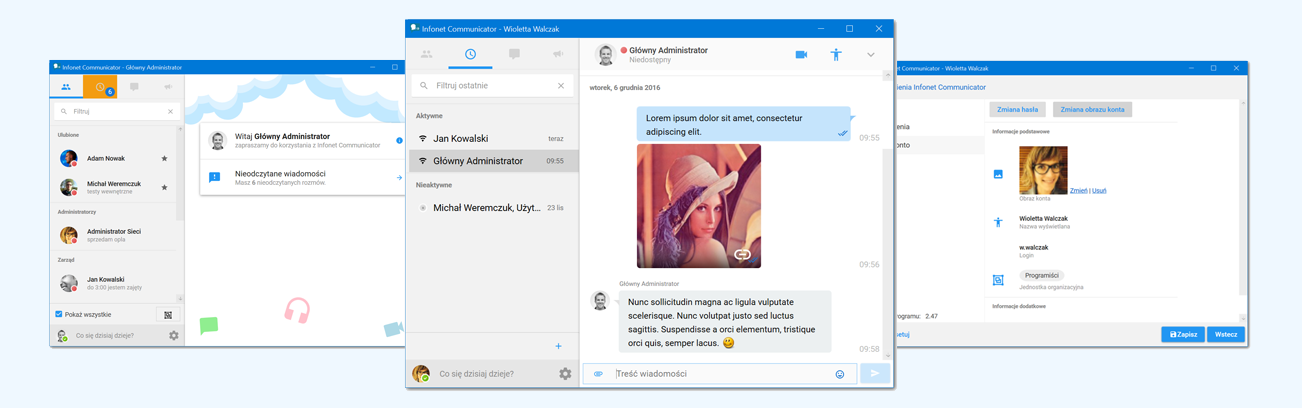
\includegraphics[width=\textwidth]{komunikator.PNG}
        \caption{Wygląd komunikatora}
        \label{fig:my_label}
    \end{figure}
\end{frame}

\begin{frame}{Komunikator}
    Fuknkcje komunikatora:
    \begin{itemize}
        \item Powiadomienia i komunikaty powitalne
        \item Zarządzanie użytkownikami
        \item Konfiguracja
        
    \end{itemize}
\end{frame}

\begin{frame}{Projektowanie sieci komputerowych}
   GNS3 jest używany przez setki tysięcy inżynierów sieciowych na całym świecie do emulacji, konfiguracji, testowania i rozwiązywania problemów z sieciami wirtualnymi i rzeczywistymi. GNS3 pozwala na uruchomienie małej topologii składającej się tylko z kilku urządzeń na twoim laptopie, do tych, które mają wiele urządzeń hostowanych na wielu serwerach lub nawet w chmurze.
\end{frame}

\begin{frame}{Czym jest GNS3}
    GNS3 składa się z dwóch komponentów oprogramowania: 
    \begin{itemize}
        \item  Oprogramowanie GNS3-all-in-one (GUI)
        \item Maszyna wirtualna GNS3 (VM)
    \end{itemize}
    GNS3-all-in-one: Jest to część kliencka GNS3 i jest graficznym interfejsem użytkownika (GUI). Instalujesz oprogramowanie typu „all-in-one” na lokalnym komputerze (Windows, MAC, Linux) i tworzysz swoje topologie za pomocą tego oprogramowania.
\end{frame}

\begin{frame}{Zalety GNS3}
    \begin{itemize}
        \item Darmowe oprogramowanie
        \item Oprogramowanie Open Source
        \item Brak miesięcznych lub rocznych opłat licencyjnych
        \item Brak ograniczenia liczby obsługiwanych urządzeń (jedynym ograniczeniem jest sprzęt: procesor i pamięć)
        \item Dostępne do pobrania, bezpłatne, wstępnie skonfigurowane i zoptymalizowane urządzenia ułatwiające wdrażanie do sieci
    \end{itemize}
\end{frame}

\begin{frame}{Wady GNS3}
    \begin{itemize}
        \item Nie jest to samodzielny pakiet, ale wymaga lokalnej instalacji oprogramowania (GUI).
        \item Konfiguracja i ograniczenia komputera mogą mieć wpływ na GNS3 ze względu na lokalną instalację (ustawienia zapory i zabezpieczeń, firmowe zasady dotyczące laptopów itp.).
    \end{itemize}
\end{frame}

\begin{frame}{Cisco Packet Tracer jako konkurencja dla GNS3}
    Cisco Packet Tracer - oficjalny produkt Cisco dla studentów Cisco Academy, który symuluje sieci Cisco. Nie emuluje sprzętu Cisco ani nie obsługuje rzeczywistych obrazów od Cisco lub innych dostawców.
\end{frame}

\begin{frame}{Szyfrowanie nośników danych}
     Rodzaje nośników danych:\\
     \begin{itemize}
         \item nośniki USB
        \item płyty
        \item partycje
        \item przestrzenie w chmuarch
     \end{itemize}
   
\end{frame}

\begin{frame}{Niebezpieczeństwa}
    W przypadku kradzieży komputera, złodziej ma dostęp do wszystkich danych.
    Zabezpieczenie systemu hasłem, w tym wypadku jest niewystarczające. Można wykorzystystać następujące metody, aby dostać się do danych:\\
    
    \begin{itemize}
        \item wyciągniecie dysku i przełożenie do innego komputera
        \item złamanie hasła
        \item wykorzystanie pendriva z systemem operacyjnym
    \end{itemize}
   
    
\end{frame}

\begin{frame}{Szyfrowanie nośników danych}
Szyfrowanie całego dysku czy wybranej przestrzeni
\newline
    \begin{figure}[H!]
        \centering
        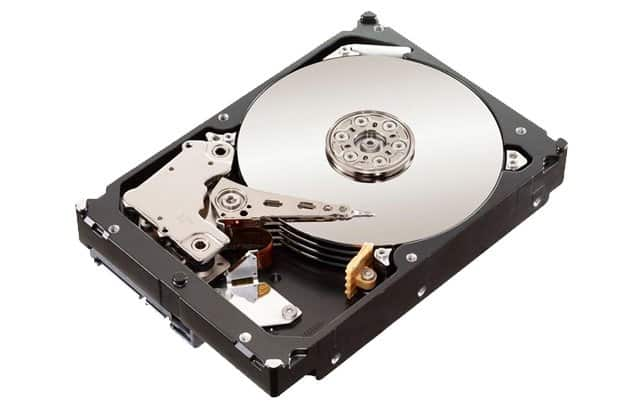
\includegraphics[width=\textwidth]{Dysk.jpg}
        \label{fig:my_label}
    \end{figure}
\end{frame}


\begin{frame}{Sposoby szyfrowania}
    Bitlocker - oprogramowanie wbudowane w system Windows\\
    TPM - Trusted Platform Module, układ scalony wbudowany w płytę główną komputera\\
    VeraCrypt - otwarte oprogramowanie
    
\end{frame}

\end{document}
